%==============================================================================
% kodovani: UTF-8 (zmena prikazem iconv, recode nebo cstocs)
% encoding: UTF-8 (you can change it by command iconv, recode or cstocs)
%------------------------------------------------------------------------------
% zpracování / processing: make, make pdf, make clean
%==============================================================================

\documentclass[english]{fitthesis}

%---rm---------------
\renewcommand{\rmdefault}{lmr}%zavede Latin Modern Roman jako rm / set Latin Modern Roman as rm
%---sf---------------
\renewcommand{\sfdefault}{qhv}%zavede TeX Gyre Heros jako sf
%---tt------------
\renewcommand{\ttdefault}{lmtt}% zavede Latin Modern tt jako tt

% vypne funkci šablony, která automaticky nahrazuje uvozovky,
% aby nebyly prováděny nevhodné náhrady v popisech API apod.
% disables function of the template which replaces quotation marks
% to avoid unnecessary replacements in the API descriptions etc.
\csdoublequotesoff



\usepackage{url}
\usepackage{amsmath}
\usepackage{blkarray}


% =======================================================================
% balíček "hyperref" vytváří klikací odkazy v pdf, pokud tedy použijeme pdflatex
% problém je, že balíček hyperref musí být uveden jako poslední, takže nemůže
% být v šabloně
% "hyperref" package create clickable links in pdf if you are using pdflatex.
% Problem is that this package have to be introduced as the last one so it 
% can not be placed in the template file.
\ifWis
\ifx\pdfoutput\undefined % nejedeme pod pdflatexem / we are not using pdflatex
\else
  \usepackage{color}
  \usepackage[unicode,colorlinks,hyperindex,plainpages=false,pdftex]{hyperref}
  \definecolor{hrcolor-ref}{RGB}{223,52,30}
  \definecolor{hrcolor-cite}{HTML}{2F8F00}
  \definecolor{hrcolor-urls}{HTML}{092EAB}
  \hypersetup{
	linkcolor=hrcolor-ref,
	citecolor=hrcolor-cite,
	filecolor=magenta,
	urlcolor=hrcolor-urls
  }
  \def\pdfBorderAttrs{/Border [0 0 0] }  % bez okrajů kolem odkazů / without margins around links
  \pdfcompresslevel=9
\fi
\else % pro tisk budou odkazy, na které se dá klikat, černé / for the print clickable links will be black
\ifx\pdfoutput\undefined % nejedeme pod pdflatexem / we are not using pdflatex
\else
  \usepackage{color}
  \usepackage[unicode,colorlinks,hyperindex,plainpages=false,pdftex,urlcolor=black,linkcolor=black,citecolor=black]{hyperref}
  \definecolor{links}{rgb}{0,0,0}
  \definecolor{anchors}{rgb}{0,0,0}
  \def\AnchorColor{anchors}
  \def\LinkColor{links}
  \def\pdfBorderAttrs{/Border [0 0 0] } % bez okrajů kolem odkazů / without margins around links
  \pdfcompresslevel=9
\fi
\fi
% Řešení problému, kdy klikací odkazy na obrázky vedou za obrázek
% This solves the problems with links which leads after the picture
\usepackage[all]{hypcap}

% Informace o práci/projektu / Information about the thesis
%---------------------------------------------------------------------------
\projectinfo{
  %Prace / Thesis
  project={SP},            %typ práce SP  / thesis type (SP = PDS project)
  year={},             % rok odevzdání / year of submission
  date={\today},             % datum odevzdání / submission date
  %Nazev prace / thesis title
  title.en={Log File Analysis and Anomaly Detection},
  title.cs={Data Communications, Computer Networks and Protocols \--- Project},
  title.length={14.5cm}, % nastavení délky bloku s titulkem pro úpravu zalomení řádku (lze definovat zde nebo níže) / setting the length of a block with a thesis title for adjusting a line break (can be defined here or below)
  %sectitle.length={14.5cm}, % nastavení délky bloku s druhým titulkem pro úpravu zalomení řádku (lze definovat zde nebo níže) / setting the length of a block with a second thesis title for adjusting a line break (can be defined here or below)
  %dectitle.length={14.5cm}, % nastavení délky bloku s titulkem nad prohlášením pro úpravu zalomení řádku (lze definovat zde nebo níže) / setting the length of a block with a thesis title above declaration for adjusting a line break (can be defined here or below)
  %Autor / Author
  author.name={Peter},   % jméno autora / author name
  author.surname={Koprda},   % příjmení autora / author surname 
  author.title.p={Bc.}, % titul před jménem (nepovinné) / title before the name (optional)
  %author.title.a={Ph.D.}, % titul za jménem (nepovinné) / title after the name (optional)
  %faculty={FIT}, % FIT/FEKT/FSI/FA/FCH/FP/FAST/FAVU/USI/DEF
  faculty.cs={Fakulta informačních technologií}, % Fakulta v češtině - pro využití této položky výše zvolte fakultu DEF / Faculty in Czech - for use of this entry select DEF above
  faculty.en={Faculty of Information Technology}, % Fakulta v angličtině - pro využití této položky výše zvolte fakultu DEF / Faculty in English - for use of this entry select DEF above
}


% nastavení délky bloku s titulkem pro úpravu zalomení řádku - lze definovat zde nebo výše / setting the length of a block with a thesis title for adjusting a line break - can be defined here or above
%\titlelength{14.5cm}
% nastavení délky bloku s druhým titulkem pro úpravu zalomení řádku - lze definovat zde nebo výše / setting the length of a block with a second thesis title for adjusting a line break - can be defined here or above
%\sectitlelength{14.5cm}
% nastavení délky bloku s titulkem nad prohlášením pro úpravu zalomení řádku - lze definovat zde nebo výše / setting the length of a block with a thesis title above declaration for adjusting a line break - can be defined here or above
%\dectitlelength{14.5cm}

% řeší první/poslední řádek odstavce na předchozí/následující stránce
% solves first/last row of the paragraph on the previous/next page
\clubpenalty=10000
\widowpenalty=10000

% checklist
\newlist{checklist}{itemize}{1}
\setlist[checklist]{label=$\square$}

% Nechcete-li, aby se u oboustranného tisku roztahovaly mezery pro zaplnění stránky, odkomentujte následující řádek / If you do not want enlarged spacing for filling of the pages in case of duplex printing, uncomment the following line
% \raggedbottom

\begin{document}
  % Vysazeni titulnich stran / Typesetting of the title pages
  % ----------------------------------------------
  \maketitle
  % Obsah
  % ----------------------------------------------
  \setlength{\parskip}{0pt}

  {\hypersetup{hidelinks}\tableofcontents}
  

  \ifODSAZ
    \setlength{\parskip}{0.5\bigskipamount}
  \else
    \setlength{\parskip}{0pt}
  \fi

  % vynechani stranky v oboustrannem rezimu
  % Skip the page in the two-sided mode
  \iftwoside
    \cleardoublepage
  \fi

  % Text prace / Thesis text
  % ----------------------------------------------
  \chapter{Introduction}
\label{chap:introduction}


\chapter{Log file analysis}
\label{chap:log-analysis}

Log file analysis~\cite{hulshof2005logfile} is a basic method that offers a significant understanding of cognitive procedures and interaction with computer applications. This process includes the collection, examination, and explanation of information from log files. By employing these techniques, we can understand the behavior of the system, pinpoint problems, and spot irregularities. This chapter is designed to outline the objectives of log file analysis and the techniques that can be employed in the process, particularly in the realm of anomaly detection.

\section{Purpose of log file analysis}
\label{sec:purpose}
The principal aim of analyzing log files~\cite{aivalis2020logfile} is to ensure effective monitoring and management of the system by reviewing log data. This investigative process helps IT administrators and teams effectively oversee and control their systems. Through the examination of log files, they can recognize patterns, spot irregularities, resolve problems, guarantee system dependability, improve security measures, and boost system efficiency. The application of log file analysis provides an understanding of how these elements affect behavior. Monitoring user behavior is relevant in two scenarios, both practical and scientific.

In a practical context~\cite{hulshof2005logfile}, understanding the approach individuals take when interacting with a computer program can be highly beneficial. As computer usage becomes increasingly prevalent in daily life, human-computer interaction is gaining importance in various domains. With more people interacting with computer applications, there is a growing need to study user behavior and preferences. Analyzing user preferences and typical usage sequences can inform interface design modifications to align with user expectations.

In a scientific context~\cite{hulshof2005logfile}, the way individuals interact with a computer application is of substantial relevance to social science. Numerous studies in education have explored the effectiveness of computer-assisted learning. Although computers can augment the process of learning, many students face difficulties in comprehending the software utilized. A considerable amount of research has been dedicated to understanding how these elements impact learning results, particularly in the context of discovery learning via computer simulations.

\section{Steps and methods of log file analysis}
\label{sec:steps}
The log-based anomaly detection involves four steps (as shown in Figure~\ref{fig:anomaly-detection}): log collection, log parsing, feature extraction and anomaly detection~\cite{he2016expreport}.

\begin{figure}[H]
    \centering
    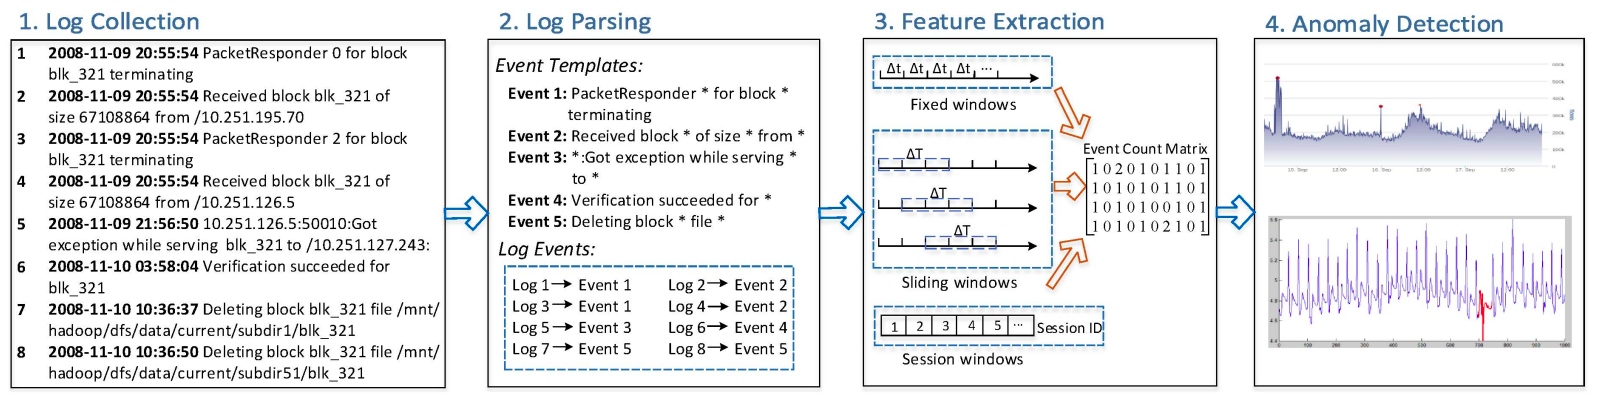
\includegraphics[width=\linewidth]{figures/anomaly-detection.png}
    \caption{Framework of anomaly detection. Retrieved from~\cite{he2016expreport}.}
    \label{fig:anomaly-detection}
\end{figure}

\subsection{Log collection}
Large-scale systems generate logs as a standard practice to record system states and runtime information. Each log record typically consists of a timestamp and a message indicating the event or action that occurred.~\cite{he2016expreport}

\subsection{Log parsing}
Log parsing aims to structure unstructured logs by extracting event templates from free-form text. Each log message is parsed into an event template consisting of a constant part and specific parameters.~\cite{he2016expreport}

There are two types of parsing methods~\cite{he2016expreport}:
\begin{enumerate}
    \item Clustering-based method \--- Computing distances between logs and then use clustering techniques to group them into clusters. The event templates are then generated from each cluster.
    \item Heuristic-based method \--- Counting the occurrences of each word at each log position. Then, frequent words are selected and combined as event candidates, from which some are chosen to be the log events.
\end{enumerate}

\subsection{Feature extraction}
The next step is to encode logs into numerical feature vectors for machine learning models. This process involves slicing the raw logs into log sequences using various grouping techniques~\cite{he2016expreport}:

\begin{enumerate}
    \item Fixed window \--- This approach relies on a timestamp that logs the time of each occurrence. Every fixed window has its own size, indicative of the time span or duration. The size of the window is represented by a constant value \--- $\Delta t$.
    \item Sliding window \--- Consists of two attributes: the size of the window and the size of the step. The step size is less than the window size, which results in the overlapping of various windows.
    \item Session window \--- This method is based on identifiers rather than timestamps. These identifiers serve to distinguish various execution routes in certain log data.
\end{enumerate}

Once we have generated log sequences using windowing, it allows us to construct an event count matrix X. Within each log sequence, we count the frequency of each log event to create the event count vector. To illustrate, [0, 0, 2, 3, 0, 1, 0] means that event 3 took place twice, and event 4 occurred three times.~\cite{he2016expreport}

\subsection{Anomaly detection}
Once the feature matrix is prepared, it can be inserted into machine learning models for training. These models are then used to generate a model specifically designed for anomaly detection.~\cite{he2016expreport}

There are various methods that can be used for anomaly detection; some of them use supervised learning (machine learning task of creating a model based on training data that has been labeled), some of them unsupervised learning (machine learning task of creating a model based on training data that has not been labeled)~\cite{he2016expreport}. For example:
\begin{itemize}
    \item \emph{Logistic regression} (supervised anomaly detection) \--- This technique is extensively utilized for classification. Logistic regression calculates the likelihood \texttt{p} for all potential states. When a new instance appears, the logistic function is capable of computing the likelihood \texttt{p} for all potential states. For anomaly detection, log sequences create event count vectors, forming instances with labels. Training builds a logistic regression model, applied to testing instances to determine anomalies~\cite{he2016expreport}.
    \item \emph{Decision Tree} (supervised anomaly detection) \--- This method uses branching to describe the expected scenario for each instance. The decision tree is built from the top downwards, utilizing training data~\cite{he2016expreport}.
    \item \emph{SVM} (supervised anomaly detection) \--- The approach of the Support Vector Machine (SVM) is to non-linearly project vectors into a feature space of very high dimensionality, with the aim of creating a linear decision boundary (hyperplane) within this feature space~\cite{wang2017research}. In the context of anomaly detection using SVM, a new instance would be identified as an anomaly if it is positioned above the hyperplane, but it would be classified as normal if it is not~\cite{he2016expreport}.
    \item \emph{Log Clustering} (unsupervised anomaly detection) \--- In this method, we organize log sequences into clusters based on their similarities. By clustering logs, we can efficiently represent different categories of events within the system. At the stage of initializing the knowledge base, logs are transformed into vectors and grouped into sets of normal and abnormal events. Vectors that represent the usual behavior are identified for each cluster. In the process of online learning, new logs are incorporated, and the clusters are progressively updated. When detecting anomalies, the distances to the representative vectors are calculated, and anomalies are marked if they surpass certain thresholds~\cite{egersdoerfer2022clusterlog}.
    \item \emph{PCA} (unsupervised anomaly detection) \--- Principal Component Analysis (PCA) is a statistical method that is commonly used to reduce dimensions. The fundamental concept involves mapping high-dimensional data onto a new coordinate system made up of \emph{k} principal components. PCA determines the \emph{k} principal components by identifying components that capture the greatest variance in the high-dimensional data. For the purpose of anomaly detection, every log sequence is transformed into an event count vector. Subsequently, PCA is utilized to discover relationships among the dimensions of these event count vectors~\cite{he2016expreport}.
\end{itemize}


\chapter{Log dataset analysis}
\label{chap:analysis}
This chapter dives deep into the examination of a chosen log dataset for this project. The dataset under consideration is derived from the ZooKeeper service\footnote{\url{https://zookeeper.apache.org}} \--- a centralized platform responsible for the preservation of configuration data, naming, offering distributed synchronization, and facilitating group services. The log dataset is constructed by compiling logs from the ZooKeeper service across a network of 32 machines, spanning nearly a 27-day timeframe~\cite{zhu2023loghub}.

\section{Dataset overview}
\label{sec:overview}
The chosen dataset possesses a size of 9.95 MB and contains 74 380 lines~\cite{zhu2023loghub}. Given that it lacks labels, only unsupervised learning techniques can be employed for machine learning methods. This dataset is downloaded from the Github page\footnote{\url{https://github.com/logpai/loghub}}, which provides links to a~variety of log datasets. The chosen log dataset consists of unprocessed log entries; however, it is possible to find structured 2000 log entries (for example for ZooKeeper service log\footnote{\url{https://github.com/logpai/loghub/blob/master/Zookeeper/Zookeeper_2k.log_structured.csv}}). This can give us a deeper overview of the selected data set.

\lstset{
    abovecaptionskip=10pt,
    caption={A sample from ZooKeeper log dataset.},
    label={lst:zookeeper},
    basicstyle=\ttfamily\normalsize\bfseries,
    xleftmargin=.005\textwidth, xrightmargin=.2\textwidth,
}
\begin{lstlisting}
2015-07-29 17:41:41,648 - INFO  [main:QuorumPeer@913] - tickTime set to 2000
2015-07-29 17:41:41,738 - WARN [WorkerSender[myid=1]:QuorumCnxManager@368]
- Cannot open channel to 3 at election address /10.10.34.13:3888
2015-07-29 23:44:23,842 - ERROR [CommitProcessor:2:NIOServerCnxn@180]
- Unexpected Exception:
\end{lstlisting}

A sample from ZooKeeper log dataset is shown in Listing~\ref{lst:zookeeper}. This sample contains three different log entries. Each log record contains several elements. The first two elements (``DateTime'' and ``Log level'') can be easily parsed. However, in order to extract the ``Node'', ``Component'' and ``Id'' elements, it is required to interpret the string that is positioned between the log level element and the final hyphen ('-') in the log record. This is demonstrated in Listing~\ref{lst:zookeeper} \--- \texttt{[main:QuorumPeer@913]} in the first log record, \texttt{[WorkerSender[myid=1]:QuorumCnxManager@368]} in the second log record, and \texttt{[CommitProcessor:2:NIOServerCnxn@180]} in the final log record. Table~\ref{tab:before-parse} shows how it looks before parsing that element into three elements and Table~\ref{tab:after-parse} how it looks after parsing that element into three elements.

\begin{table}[H]
\centering
\caption{Before parsing}
\label{tab:before-parse}
\vspace*{2mm}
\begin{tabular}{|cll|}
\hline
\multicolumn{3}{|c|}{\textbf{Log elements}} \\ \hline
\multicolumn{3}{|c|}{{[}main:QuorumPeer@913{]}} \\ \hline
\multicolumn{3}{|c|}{{[}WorkerSender{[}myid=1{]}:QuorumCnxManager@368{]}} \\ \hline
\multicolumn{3}{|c|}{{[}CommitProcessor:2:NIOServerCnxn@180{]}} \\ \hline
\end{tabular}
\end{table}

\begin{table}[H]
\centering
\caption{After parsing}
\label{tab:after-parse}
\vspace*{2mm}
\begin{tabular}{|c|c|c|}
\hline
\textbf{Node} & \textbf{Component} & \textbf{Id} \\ \hline
main & QuorumPeer & 913 \\ \hline
WorkerSender{[}myid=1{]} & QuorumCnxManager & 368 \\ \hline
\multicolumn{1}{|l|}{CommitProcessor} & \multicolumn{1}{l|}{2:NIOServerCnxn} & \multicolumn{1}{l|}{180} \\ \hline
\end{tabular}
\vspace*{5mm}
\end{table}

\section{Elements of log entries}
Each log record has 6 different elements:
\begin{enumerate}
    \item \textbf{DateTime} \--- this indicates the date and time when the log entry was recorded. The datetime follows the pattern \texttt{YYYY-mm-dd HH:MM:SS,f}, where:
    \begin{itemize}
        \item \texttt{YYYY} represents the year in four digits,
        \item \texttt{mm} represents the month in two digits,
        \item \texttt{dd} represents the day of the month in two digits,
        \item \texttt{HH} represents the hour in 24-hour format,
        \item \texttt{MM} represents the minute in two digits,
        \item \texttt{SS} represents the second in two digits, and
        \item \texttt{f} represents the miliseconds in three digits.
    \end{itemize}
    This format provides a precise indication of when the log entry was recorded.
    
    \item \textbf{Log level} \--- this indicates the severity of the log message. The log dataset contains three categories of log messages: \texttt{INFO}, \texttt{WARN}, and \texttt{ERROR}. Each category may have a~unique role in expressing various aspects of the system's functionality and potential problems.
    
    \item \textbf{Node} \--- represents the specific node or entity within the system where the log message originated. This element in Table~\ref{tab:before-parse} is located between the first open square bracket ('[') and the first colon symbol (':').

    \item \textbf{Component} \--- specifies the particular component or module of the system associated with the log message. This element in Table~\ref{tab:before-parse} is located between the first colon symbol (':') and the ``at'' symbol ('@').

    \item \textbf{Id} \--- an identifier associated with the log record, which may be useful for tracking or correlating related events. This element in Table~\ref{tab:before-parse} is located between the ``at'' symbol and the final close square bracket (']').

    \item \textbf{Content} \--- the rest of the log message represents the actual content of the log message, providing details about an event, action, or error (e.g. in Listing~\ref{lst:zookeeper} the ``Content'' element for the first log record is ``tickTime set to 200'').
\end{enumerate}

On the Github page\footnote{\url{https://github.com/logpai/loghub/blob/master/Zookeeper/Zookeeper_2k.log_templates.csv}}, there are defined event templates for this dataset. There are 50 different event templates, each of them represents some different group of events. While these could be beneficial in identifying features for the machine learning algorithm during subsequent stages, it seems that these event templates may not be applicable to all potential log events.

\chapter{Modeling log events}
\label{chap:modeling}
In this chapter, we set out on the task of modelling log events, a crucial step in utilizing machine learning methods for log analysis and anomaly detection. We start by clarifying the complex process of data pre-processing, feature selection, and event representation, thereby establishing the foundation for building significant models.

\section{Data pre-processing}
\label{sec:data-preprocess}
The initial step that needs to be taken is the pre-processing of the data. Initially, the data is presented in a~log format, hence, it would be most beneficial to convert this data into a~two-dimensional data structure, such as a 2D array. This method makes it straightforward to ascertain the values of each log record. For instance, Listing~\ref{lst:unprocessed-log} provides an example of a raw log record:

\lstset{
    abovecaptionskip=10pt,
    caption={Example of unprocessed log record.},
    label={lst:unprocessed-log},
    basicstyle=\ttfamily\normalsize\bfseries,
    xleftmargin=.005\textwidth, xrightmargin=.2\textwidth,
}
\begin{lstlisting}
2015-07-30 18:18:02,000 - INFO  [SessionTracker:ZooKeeperServer@325] -
Expiring session 0x14ede63a5a70004, timeout of 10000ms exceeded
\end{lstlisting}

As previously pointed out in Chapter~\ref{chap:analysis}, the log records consist of 6 distinct elements. These records can be transformed, for instance, into a CSV format. This format provides a~clearer perspective on the data. In Listing~\ref{lst:csv-log}, the log elements are displayed in CSV format, separated by semicolons. The values correspond to the elements \texttt{DateTime}, 	\texttt{Log level}, \texttt{Node}, \texttt{Component}, 	\texttt{Id}, and \texttt{Content}, respectively.

\lstset{
    abovecaptionskip=10pt,
    caption={Example of log record in CSV format.},
    label={lst:csv-log},
    basicstyle=\ttfamily\normalsize\bfseries,
    xleftmargin=.005\textwidth, xrightmargin=.2\textwidth,
}
\begin{lstlisting}
2015-07-30 18:18:02.000; INFO; SessionTracker; Expiring session
0x14ede63a5a70004, timeout of 10000ms exceeded; 325;  ZooKeeperServer
\end{lstlisting}

\section{Event representation}
\label{sec:event}
Once the data is processed into CSV format, it becomes essential to rearrange these columns for the creation of log events. The best way to represent events is to use \texttt{Content} element. This element represents some type of action of the specific log record. However, it becomes imperative to cluster these messages, as identifying every single element is not the most efficient strategy, and some form of data reduction is needed. This goal can be accomplished by utilizing regular expressions that have the ability to match a variety of specific log messages. There are 5 distinct log values for this element in Listing~\ref{lst:content}. A regular expression that corresponds to these values is found on line 7.

\lstset{
    abovecaptionskip=10pt,
    caption={Example of values for \texttt{Content} element. On the line 7 is the regular expression which would match these values and \texttt{E27} is a suitable event that corresponds to this regular expression.},
    label={lst:content},
    numbers={left},
    firstnumber={1},
    stepnumber={1},
    basicstyle=\ttfamily\normalsize\bfseries,
    xleftmargin=.1\textwidth, xrightmargin=.2\textwidth,
}
\begin{lstlisting}
Expiring session 0x14ede63a5a70004, timeout of 10000ms exceeded
Expiring session 0x14ede63a5a70003, timeout of 10000ms exceeded
Expiring session 0x14ede63a5a70001, timeout of 10000ms exceeded
Expiring session 0x14ede63a5a70000, timeout of 10000ms exceeded
Expiring session 0x14ede63a5a70002, timeout of 10000ms exceeded

r'Expiring session .*, timeout of .*ms exceeded': 'E27'
\end{lstlisting}

This method allows us to generate events and assign them to the given regular expressions. Listing~\ref{lst:logrecord-event} demonstrates a processed log record from Listing~\ref{lst:unprocessed-log} following the assigning of log events to regular expressions.

\lstset{
    abovecaptionskip=10pt,
    caption={Processed log record after applying events.},
    label={lst:logrecord-event},
    numbers={none},
    basicstyle=\ttfamily\normalsize\bfseries,
    xleftmargin=.01\textwidth, xrightmargin=.2\textwidth,
}
\begin{lstlisting}
2015-07-30 18:18:02.000; INFO; SessionTracker; E27; 325; ZooKeeperServer
\end{lstlisting}


\section{Feature extraction}
\label{sec:feature}
Once log events have been assigned, it becomes possible to derive important attributes from these events. The initial input for this process is the log events themselves, while the expected output is an event count matrix. The formulation of an event count matrix requires the categorization of events into distinct groups, each of which symbolizes a~log sequence. Each log sequence contains a timestamp that records the time of occurrence for every log. Three distinct methods can be employed to formulate an event count matrix --- utilizing fixed windows, a sliding window, or a session window (previously discussed in Chapter~\ref{chap:log-analysis}). Since our dataset is not large, the most suitable strategy would be to employ the ``Fixed window'' technique. This method can be implemented by establishing a timestamp with a duration of one day. Subsequently, the number of events for each timestamp will be calculated, resulting in the generation of an event count matrix. Equation~\ref{eq:count-matrix} illustrates how the event count matrix should look. The left side of the matrix is populated with dates that serve as timestamps. It does not display the exact time, given that the selected timestamp spans a duration of one day, thus eliminating the necessity for a specific time. The top row is marked with event labels (where E1 stands for event 1, E2 for event 2, and so forth). As an illustration, on the date \texttt{2015-07-29}, the event count matrix recorded 3 instances of event 1, 45 instances of event 2, 18 instances of event 3, and 3 instances of event 4. However, on the final date represented in this matrix (\texttt{2015-08-01}), there were zero instances of events 1 through 4. This event count matrix will be appropriate for the final stage of this project, which involves the actual creation of a model for detecting anomalies.


\begin{equation}
    \begin{blockarray}{ccccc}
    &   \textbf{E1}&     \textbf{E2}&     \textbf{E3}&     \textbf{E4} \\
    \begin{block}{c(cccc)}
   \textbf{ 2015{\text -}07{\text -}29}&    3&      45&     18&     3 \\
   \textbf{ 2015{\text -}07{\text -}30}&    7&      105&    42&     7 \\
   \textbf{ 2015{\text -}07{\text -}31}&    9&      135&    54&     9 \\
   \textbf{ 2015{\text -}08{\text -}01}&    0&      0&      0&      0 \\
    \end{block}
    \end{blockarray}
    \label{eq:count-matrix}
\end{equation}

\chapter{Implementation}
\label{chap:implementation}
This chapter offers a deep understanding of the design concepts, structure, and features of the suggested tool. The tool is developed using the Python programming language\footnote{\url{https://www.python.org}} and is implemented as CLI\footnote{Command line interface} application. The proposed tool is implemented in the file \texttt{log-monitor.py}.

\chapter{Experiments}
\label{chap:experiments}


\chapter{Testing}
\label{chap:testing}


\chapter{Conclusion}
\label{chap:conclusion}

  
  % Kompilace po částech (viz výše, nutno odkomentovat)
  % Compilation piecewise (see above, it is necessary to uncomment it)
  %\subfile{projekt-01-uvod-introduction}
  % ...
  %\subfile{chapters/projekt-05-conclusion}


  % Pouzita literatura / Bibliography
  % ----------------------------------------------
\ifslovak
  \makeatletter
  \def\@openbib@code{\addcontentsline{toc}{chapter}{Literatúra}}
  \makeatother
  \bibliographystyle{bib-styles/Pysny/skplain}
\else
  \ifczech
    \makeatletter
    \def\@openbib@code{\addcontentsline{toc}{chapter}{Literatura}}
    \makeatother
    \bibliographystyle{bib-styles/Pysny/czplain}
  \else 
    \makeatletter
    \def\@openbib@code{\addcontentsline{toc}{chapter}{Bibliography}}
    \makeatother
    \bibliographystyle{bib-styles/Pysny/enplain}
  %  \bibliographystyle{alpha}
  \fi
\fi
  \begin{flushleft}
  \bibliography{project-pds-bibliography}
  \end{flushleft}

  % vynechani stranky v oboustrannem rezimu
  % Skip the page in the two-sided mode
  \iftwoside
    \cleardoublepage
  \fi


% vynechani stranky v oboustrannem rezimu
% Skip the page in the two-sided mode
%\iftwoside
%  \cleardoublepage
%\fi
  
  \ifODSAZ
    \setlength{\parskip}{0.5\bigskipamount}
  \else
    \setlength{\parskip}{0pt}
  \fi
  
  % vynechani stranky v oboustrannem rezimu
  \iftwoside
    \cleardoublepage
  \fi
  
\end{document}
